\section{State of the Art for Discontinuous Galerkin Methods} % for the \MA equation}

The most natural attempt for a formulation of a DG method is to exploit the equations
\begin{align}
	\myIntX {\Omega} {\mydet {D^2 u} v} = \myIntX \Omega {fv} \qquad \text{ for all test functions } v. \label{eq: naiv ansatz}
\end{align}

In 2008 B\"ohmer investigated this ansatz for $C^1$ elements in \cite{Boehmer2008}. He derives a general $C^1$ method including statements on its stability and consistency. 
He is able to reduce the convergence analysis to the linearised case \cite[Section 9]{Boehmer2008}, and discovers even a connection between the weak and strong linearised forms: For his chosen elements these operators even coincide meaning the diagram in Figure \ref{fig: fe diagram} commutes.
\begin{figure}[H]
			\begin{center}
		\usetikzlibrary{matrix}

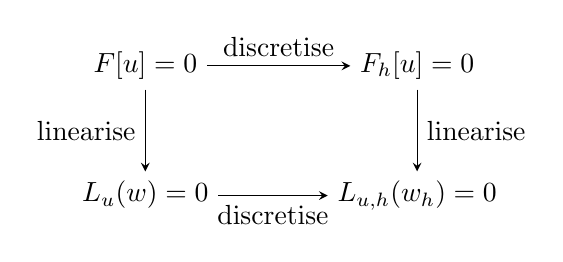
\begin{tikzpicture}[scale =2]
  \matrix (m) [matrix of math nodes,row sep=3em,column sep=4em,minimum width=2em]
  {
     F[u]=0 & F_h[u] =0 \\
     L_u(w) =0 & L_{u,h}(w_h)=0 \\};
  \path[-stealth]
    (m-1-1) edge node [left] {linearise} (m-2-1)
            edge node [above] {discretise} (m-1-2)
    (m-2-1.east|-m-2-2) edge node [below] {discretise} (m-2-2)
    (m-1-2) edge node [right] {linearise} (m-2-2);
\end{tikzpicture}
		\end{center}

	\caption{An abstract commuting diagram about the relation between weak and strong linear operators.\\ The analytical \MA operator is hereby denoted by $F:=\detHess u$ and its linearisation $L_u(w) = -\nabla \cdot (\cofHess u \nabla w)$, compare \ref{sec: linearisation}. $F_h[u]=0$ denots the discretised formulation, for B\"ohmer's method this is given by \eqref{eq: naiv ansatz}. The diagram is taken of \cite[Fig 2.2]{FGN2013}}
	\label{fig: fe diagram}	
\end{figure}
However, this formulation has two major disadvantages. 
At first we cannot throw the high derivatives onto the test functions using integration by parts, thus we we have to handle the high derivatives. Secondly \eqref{eq: naiv ansatz} seems to work only for test and ansatz functions contained in $C^1(\Omega)$ whereas usual finite elements are contained in $C^0$. B\"ohmer claims \quoting{ We require FEs in $C^1$, since for FEs in $C^0$ we did not see a possibility to handle the interior variational crimes. The standard interplay between the weak and strong form is impossible for fully nonlinear problems and \emph{excludes, e.g. discontinuous Galerkin methods.}}\cite[p.1214]{Boehmer2008}.

Indeed the diagram in Figure \ref{fig: fe diagram} does not commute for less regular spaces and Brenner et alter make this inconsistency responsible for the failure of $C^0$ methods\cite{BGN+2011}. Their idea is to improve the discretised formulation by adding DG terms to force consistency between the linearisation of the discrete problem and the linearisation of the continuous problem.

\subsection{A $C^0$ Penalty Method }\label{sec: Brenner method}

Given zero boundary conditions the linearisation of the left-hand side of \eqref{eq: naiv ansatz} can be derived exactly as in the proof of theorem \ref{thm: linearisation} leading to the bilinear form
\begin{align}
\langle L_{u,h}(w_h),v_h\rangle =& \myIntX {\Omega} {\nabla \cdot \left( \mycof {D^2 u_h } \nabla w_h \right) v_h}
%=& \int_{\Omega} \left( \mycof {D^2 u_h } \nabla w_h \right) \nabla v_h. 
\label{eq: linearOperator}
\end{align}

Now we analyse the variational form of the linearisation of the \MA equation. Due to integration by parts it holds
\begin{align*}
  \myIntX  T { \nabla \cdot (\mycof{D^2 u_h} \nabla w_h) v_h}
  	=& -\myIntX  T { (\mycof{D^2 u_h} \nabla w_h) \nabla v_h} \\
  	&	+ \myIntS  {\partial T} { (\mycof{D^2 u_h} \nabla w_h) v_h}.
\end{align*}
Summing over the whole triangulation it becomes
\begin{align*}
  \myIntX  \Omega { \nabla \cdot (\mycof{D^2 u_h} \nabla w_h) v_h}
  	=& -\myIntX  \Omega { (\mycof{D^2 u_h} \nabla w_h) \nabla v_h} \\
  	 &	+ \sum_{e \in \edgesi} \myIntS e { \llbracket \{\{\mycof{D^2 u_h} \}\} \nabla w_h\rrbracket v_h}.
\end{align*}
Considering the last identity the variational form of the linearisation reads
\begin{align}
	\langle L^L_{u}(w_h),v_h\rangle 
	    =&- \sum_{T \in \triang}  \myIntX  T { \nabla \cdot (\mycof{D^2 u_h} \nabla w_h) v_h} \nonumber \\
	    	&+ \sum_{e \in \edges} \myIntS e { \llbracket \{\{\mycof{D^2 u_h} \}\} \nabla w_h\rrbracket v_h} \nonumber \\
	    	&+ \sum_{e \in \edges} \myIntS e { \llbracket \{\{\mycof{D^2 u_h} \}\} \nabla v_h\rrbracket w_h} \label{eq: var of linearisation}
\end{align}
Plugging the terms missing in \eqref{eq: linearOperator} but appearing in \eqref{eq: var of linearisation} into the original naive ansatz \eqref{eq: naiv ansatz} and adding further terms to enforce weak boundary conditions they end up with the problem: Find $u_h \in V_h$ such that
\begin{align}
\begin{split}
	&\myIntX {\Omega} {(f-\mydet {D^2_h u_h} v} 
	+ \sum_{e \in \edgesi} \myIntS e { \llbracket \{\{\mycof{D^2 u_h} \}\} \nabla u_h\rrbracket v_h} \\
	&- \sum_{e \in \edgesb} \myIntS e { \llbracket \{\{\mycof{D^2 u_h} \}\} \nabla v_h\rrbracket (u_h -g)} 
	+ \sigma  \sum_{e \in \edgesb} \frac 1 {h_e} \myIntS e { (u_h -g)}  = 0 \; \forall v_h \in V_h \label{eq: brenner method}
\end{split}
\end{align}
They choose their ansatz and test space $V_h$ to be the space of continuous functionous being piecewise polynomials up to degree $k$ for a $k \geq 3$. For their analysis they assume the \MA problem has strictly convex solution $u\in H^s(\Omega)$ for $s>3$. %Then they are able to derive stability of the linearisation of their operator. 

The key for the convergence proof is a fixed point argument: They expanded the mapping given by the right-hand side of \eqref{eq: brenner method} to a linearisation at the solution $u$ (cf. \eqref{eq: var of linearisation}  and a remaining quadratic mapping $R$. That means they can write \eqref{eq: brenner method} by 
\begin{align}
	\bilin {F (u+w)} v = \bilin {L^L_{u_h}w} v + \bilin {Rw} v. \label{eq: brenner entwicklung}
\end{align}
With this at their hand they define a mapping $\mathcal M_h$. The choice of their $\mathcal M$ has two important properties. At first, its fixed point is the solution to their finite element. At second, $\mathcal M$ is chosen in such a way that its contraction property almost follows directly from a contraction property of $R$.
Using the Banach fixed point theorem they can show existence of a fixed point of $\mathcal M$ in $V_h$ and locate it within an arbitrary small set. Fortunately, this yields an error estimate for their numerical solution:
\todo{reference auf später}
\begin{theorem}[Error Estimate{\cite[Theorem 3.1 and 3.2]{BGN+2011}}]\label{thm: error estimate brenner}
	There exists an $h_0(\sigma) > 0$ such that for $h \leq h_0(\sigma)$ there exists a solution $u_h$ to the penalty method \eqref{eq: brenner method}. Moreover, if $u \in W^{s,\infty}$ with $s>3$ then holds
	\begin{align*}
%		\norm{u-u_h}_{1,h} \lesssim (1+\sigma) h^{l-1} \norm{u}_H
		\norm{u-u_h}_{L^2(\Omega)} \lesssim (1+\sigma)^2 
		                        \left(h^{l} \norm{u}_{H^l(\Omega)} + (1+ | \ln h |^{\frac 1 2 }) h^{2(l-2)} \norm{u}_{H^l(\Omega)} \right)
	\end{align*}
where $l=\min\{k+1,s\}$. 
\end{theorem}
This theorem ensure almost optimal convergence orders provided a smooth solution. Although there analysis assumes the polynomial degree $k\geq 3$ their numerical results also suggest optimal convergence rates for $k=2$.\\
However, their approach has a drawback. In order to find $u_h$ one has to solve the from \eqref{eq: brenner method} resulting nonlinear system. Brenner et alt. make use of Newton's method in the numerical results to solve their example problems. For a good initial guess they inquire a vanishing moments method which internally again solves a nonlinear systems based on a Newton's method. The starting point required of this internal Newton solver is calculated using a nested iteration.

Neilan claims when presenting another DG method in \cite{Neilan2014} that this methods fails to converge for the test case $u = -\sqrt{2 - x_1^2 - x_2^2 }$ and $f = \frac 2 {{2 - x_1^2 - x_2^2}^2}$ which lacks $H^2$ regularity and our computations confirm this result, see also test \ref{test sqrt}. In chapter \ref{ch:NumericalResults} we provide some numerical experiments for a nested iteration variant of this method. Generally speaking, the presented method is more appropriate for classical solutions, Brenner et alt. say they plan to address less regular solution in future work. 


\subsection{A Finite Element Method based on a Discrete Hessian} \label{subsec: disrete Hessian} \label{sec: FEM discrete Hessian}

Shortly Neilan generalised in \cite{Neilan2014} a finite element method of Lakkis and Pryer presented in \cite{LP2011}.
The crux of this idea is the notion of a \emph{discrete Hessian}. 
While the real Hessian fulfills due to integration by parts as we have seen in Lemma \ref{la: integration by parts Frobenius}
	\begin{align}
		\myIntX  \Omega { (D^2 u : B)} = 
			- \myIntX  \Omega { \left(\nabla \cdot B\right) \cdot \nabla u} 
			+ \myIntS {\partial \Omega}  {B \nabla u \mathbf {n}} \qquad \forall B \in [H^1(\Omega)]^{d \times d}, \label{eq: part int hessian}
	\end{align}
often the piecewise derived Hessian $D_h^2 v$ of $ v \in V_h$ for less regular ansatz spaces $V_h$ does not inherit this property. Considering that most weak formulations base on a integration by parts approach, the idea of a discretisation of the Hessian retaining this quality is standing to reason. To create this discretisation Neilan carries the integration from \eqref{eq: part int hessian} piecewise on every triangle out and rewrites the edge terms by a combination of jump and averages as usual leading to
	\begin{align}
		\begin{split}
		\myIntX  \Omega { (D^2 u : B)}
		=& - \myIntX  \Omega { \left(\nabla \cdot B\right) \cdot \nabla u} \\
		&+ \sum_{ e \in \edgesi} \myIntS e { \jump {\average B \nabla u }}
				+ \sum_{ e \in \edges} \myIntS e {  \jump{B \average {\nabla u} }}  \qquad \forall B \in \Sigma_h. \label{eq: part int hessian omega}
		\end{split}
	\end{align}
Observing, that the last step admits test functions $B$ only piecewise smooth, Neilan suggests the ansatz space $V_h = \mathcal{P}_h^k \cap H^1(\Omega)$ and the test space $\Sigma_h = [\mathcal{P}_h^k]^{d \times d}$.

Substituting in \eqref{eq: part int hessian omega} $\nabla u$ across the edges with its numerical counterpart, namely the numerical trace chosen as $\laverage \nabla u \raverage$ one has as predefinition of the discrete Hessian
\todo{lifting erwaehnen?}
	\begin{align}
		\myIntX  \Omega { (D_{DH}^2 u : B) }
		&= - \myIntX  \Omega { \left(\nabla \cdot B\right) \cdot \nabla u}
		+ \sum_{ e \in \edgesi} \myIntS e {  \jump {\average B \nabla u } }
				+ \sum_{ e \in \edges} \myIntS e { \jump {B \average {\nabla u} }}  \nonumber \\
		&= - \myIntX  \Omega { \left(\nabla \cdot B\right) \cdot \nabla u}
				+ \sum_{ e \in \edges} \myIntS e {  \jump{B \average {\nabla u} }}.	
	\end{align}
Applying once more integration by parts for a Frobenius product on every triangle in the right-hande side integral results in
	\begin{align}
		\myIntX  \Omega { (D_{DH}^2 u : B) }
		=& \myIntX  \Omega { D_h u: B }
			-\sum_{ e \in \edgesi} \myIntS e {  \jump {\average B  \nabla u }}
			- \sum_{ e \in \edges} \myIntS e { \jump {B \average {\nabla u} }}\nonumber \\		
			&+ \sum_{ e \in \edges} \myIntS e {  \jump {B \average {\nabla u} }}		\nonumber \\
		=& \myIntX  \Omega { D_h u: B}
			 -\sum_{ e \in \edgesi} \myIntS e {  \jump {\average B  \nabla u }	}
	\end{align}

Hence,
\begin{definition}[Discrete Hessian] \label{def: discrete Hessian}
	The discrete Hessian $D_{DH}^2 u$ of a function $u$ is the unique function satisfying
	\begin{align}
		\myIntX  \Omega { (D_{DH}^2 u : B) }
		= \myIntX  \Omega { D_h u: B}
			 -\sum_{ e \in \edgesi} \myIntS e {  \jump {\average B \nabla u }}\qquad \forall B \in \Sigma_h. \label{eq: discrete hessian}
	\end{align}
\end{definition}

Even though the Hessian is symmetric, in general the discrete Hessian is owing to the face terms not obligatory symmetric. \\
Note, that for a discontinuous $\Sigma_h$ the computations for $D_{DH}^2 u$ reduce to purely local efforts. For piecewise constant space $\Sigma_h$ the discrete Hessian $D_{DH}^2 u$ can even be computed explicitly.

The next natural step is to plug the newly deduced Hessian into the original \MA PDE resulting in the method: Find $u \in V_h$ such that

\begin{align}
		\myIntX  \Omega { \left(\mydet{D_{DH}^2 u} - f \right) v} = 0 \qquad \forall v \in V_h \label{eq: neilan eq1}
\end{align}
where
	\begin{align}
		\myIntX  \Omega { (D_{DH}^2 u : B) }
		= \myIntX  \Omega { D_h u: B}
			 -\sum_{ e \in \edgesi} \myIntS e {  \jump {\average B \nabla u }}\qquad \forall B \in \Sigma_h. \tag{\ref{eq: discrete hessian}}
	\end{align}

Neilan proceeds analogously to the prove of the well-posedness of the method mentioned in the previous section \ref{sec: Brenner method}. At the beginning he expands the nonlinear mapping at the solution $u$ and then he uses an analogous mapping $\mathcal M$ to obtaining convergence with the Banach fixed point theorem. Note, that the new notion of an discrete Hessian makes the estimates of this unconventional linearisation hard to handle. The linearisation used in the other $C^0$ penalty method is more common and hence the arguments for deriving estimates for the linear part were already well known.
He ends up with the following error estimation:
\begin{theorem}
	Let $u$ be the convex solution to the \MA equation and suppose $u$ to be in the Hölder space $C^{k+3,\alpha}$ for $\alpha \in (0,1)$ and the polynomial degree $k\geq3$. Then there exists a $h_0$ such that for all $h > h_0$ there exists a solution $u_h \in V_h$ to \eqref{eq: neilan eq1} with
	\[
		\norm{u-u_h}_{1,h} \leq C h^k
	\]
	where $C$ is a constant independent on $h$ and $\norm{\cdot }_{1,h}$ is the discrete semi-norm 
	\[
		\norm{v}_{1,h}^2 = \norm {\nabla v }^2_{L^2(\Omega)} + \sum_{e \in \edges} |e| \norm {\average {\nabla v}}^2_{L^2(\Omega)}.
	\]
\end{theorem}

Albeit he cannot prove any further relaxations, his numerical experiments suggest that his method even works for smaller polynomial degrees and problems which's solution lacks $H^2$ regularity. 
\\However, for $k=1$ he has to add an additional penalty term to obtain convergence. Thus, for piecewise affine functions he instead solves:
\begin{align}
		\myIntX  \Omega { \left(\mydet{D_{DH}^2 u} - f \right) v} 
			+ \eta \sum_{e \in \edgesi} |e| \myIntS e { \jump{ \nabla u_h} \jump{\nabla v}}
		= 0 \qquad \forall v \in V_h \label{eq: neilan eq1 + jump}
\end{align}
where
	\begin{align*}
		\myIntX  \Omega { (D_{DH}^2 u : B) }
		= \myIntX  \Omega { D_h u: B}
			 -\sum_{ e \in \edgesi} \myIntS e {  \jump {\average B \nabla u }}\qquad \forall B \in \Sigma_h \tag{\ref{eq: discrete hessian}}
	\end{align*}
and $\eta$ is an additional penalty parameter which Neilan takes to be 50 in his numerical tests.

We check the performance of this algorithms later in chapter \ref{ch:NumericalResults}.